This section is about the visualization of the results. The Matlab code can be found at the end of the report. Figure \ref{four} shows the temperature in the rod at four time points (namely $\tau \approx 0.5,1,1.5,2$).

\begin{figure}
\begin{center}
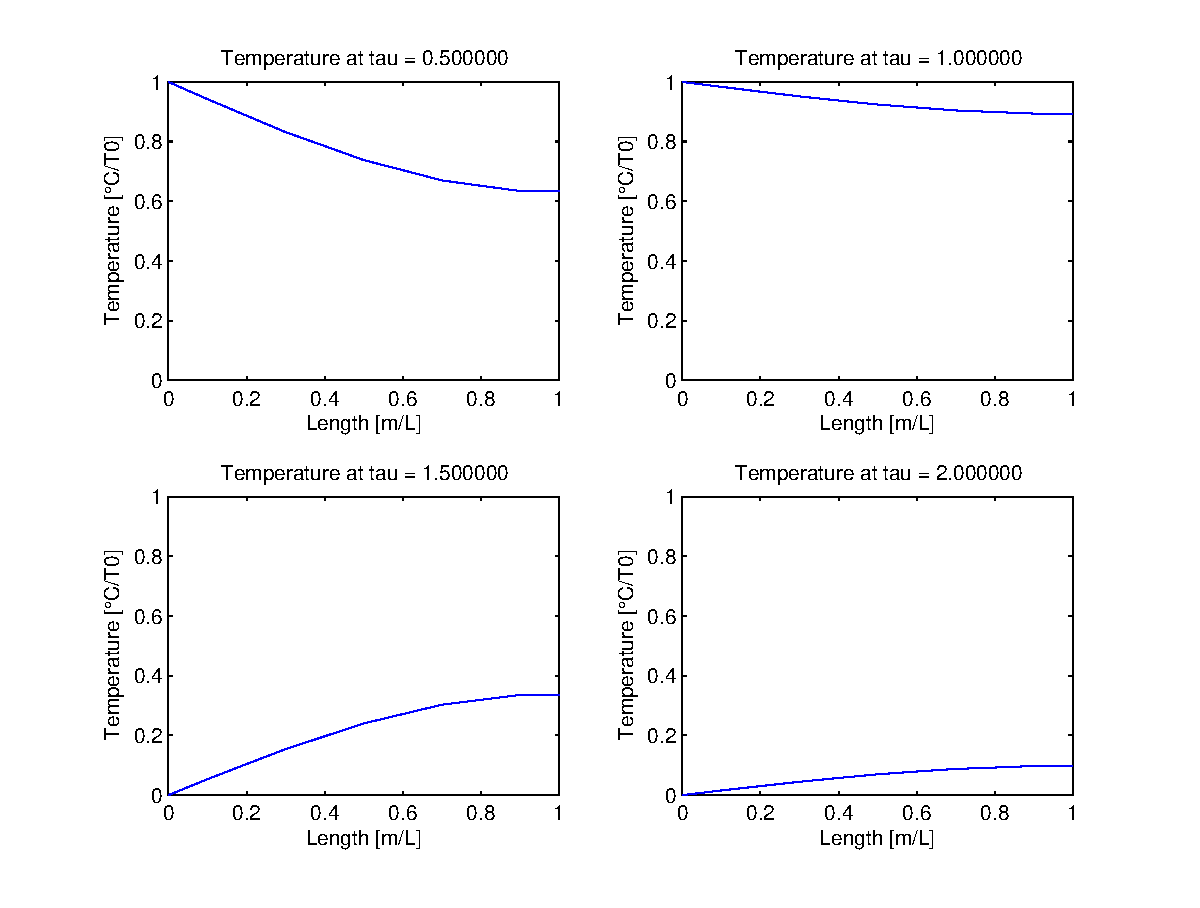
\includegraphics[width=0.9\textwidth]{four.eps}
\caption{Temperature in the rod at different times}
\label{four}
\end{center}
\end{figure}

We can notice that the boundary condition is fulfilled (as it always should be). The temperature rises until $\tau = 1$ and then starts decreasing, as it is expected. 

The next plot is the same as the stable one in section c). It is shown in figure \ref{stable}. This plot clearly depicts the boundary condition. As for the initial condition, the discretization of the $x$-axis has made it less obvious. We have in fact $u(0,0)=1$ and $u(0.1,0) = U_1(0) = 0$. Between the two, it should be zero but Matlab uses a linear interpolation. We can also see here that until $\tau=1$, the temperature is rising while it is decreasing afterwards.

\begin{figure}
\begin{center}
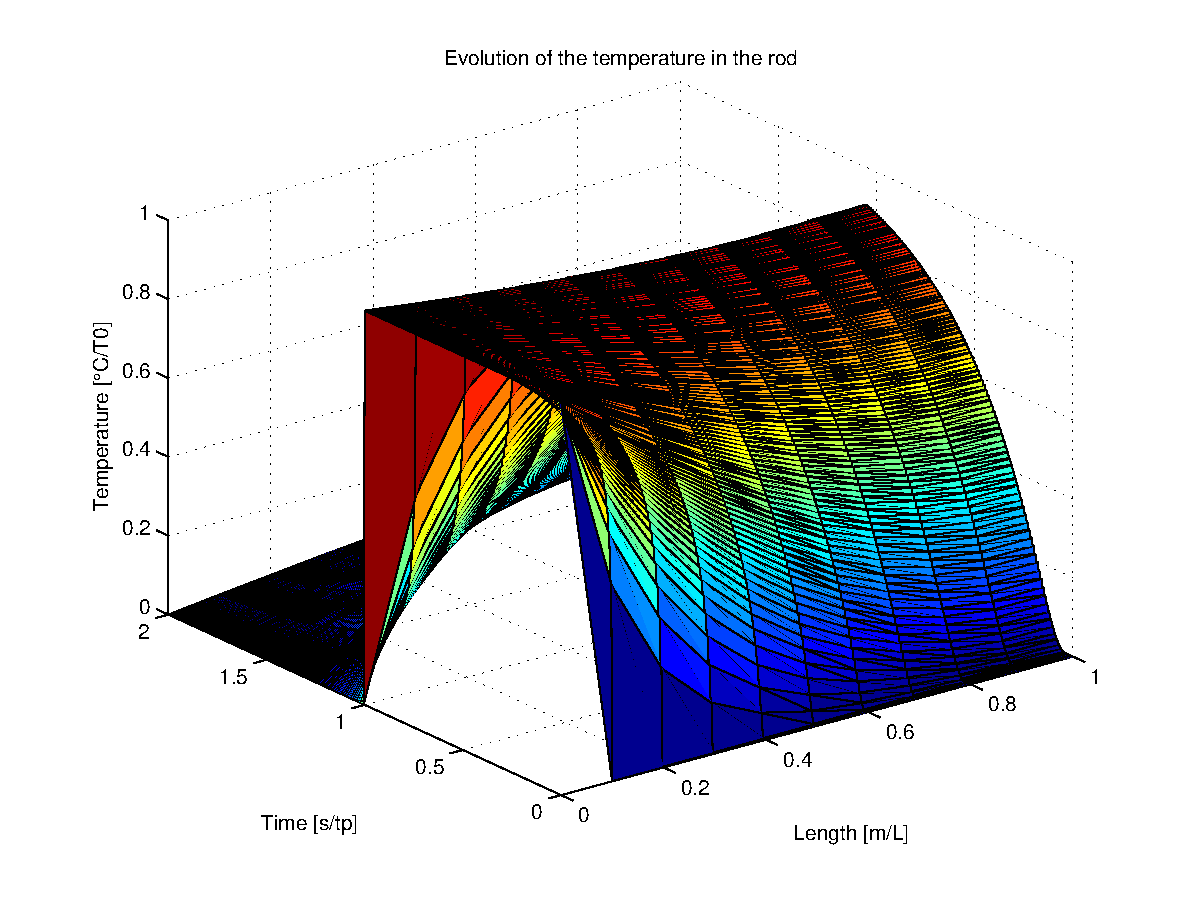
\includegraphics[width=0.7\textwidth]{stable.eps}
\caption{Temperature in the rod at any time}
\label{stable}
\end{center}
\end{figure}

\section*{Conclusion}
This report presented the solution of the very practical problem : the evolution of the temperature in a rod. This can be modelled as a parabolic PDE. To solve this PDE, we used the finite difference method to arrive at a system of ODEs. This system of ODE is stiff and a stiff method should then be used to solve it efficiently.

The stucture of the jacobian of the ODE system is really particular : it is tridiagonal (thus banded). This particularity should be taken into account when using the stiff solver (as did in section e) of the report).

\section*{MATLAB}
\lstinputlisting{graphics.m}
\lstinputlisting{tempEE.m}
\lstinputlisting{tempOde.m}